%%%%%%%%%%%%%%%%%%%%%%%%%%%%%%%%%%%%%%%
\newgeometry{left=0.8in,right=0.8in,top=1in,bottom=1in}
%%%%%%%%%%%%%%%%%%%%%%%%%%%%%%%%%%%%%%%
\chapter{Magnetic dipole moment in relativistic quantum mechanics}
\label{appendixA}
%%%%%%%%%%%%%%%%%%%%%%%%%%%%%%%%%%%%%%%
\begin{center}
Steinmetz, A., Formanek, M. \& Rafelski, J. Magnetic dipole moment in relativistic quantum mechanics. European Physical Journal A $\bb{55}$, 40 (2019). \href{https://doi.org/10.1140/epja/i2019-12715-5}{10.1140/epja/i2019-12715-5}
\end{center}

\noindent Copyright (2019) by Springer Nature. Reprinted with kind permission of The European Physical Journal (EPJ). Reprint permission for this thesis granted under \href{https://s100.copyright.com/CustomerAdmin/PLF.jsp?ref=9a7a42d0-4511-4427-8acd-73a16083772c}{License Agreement 5600921273203} License date: August 2nd, 2023.

%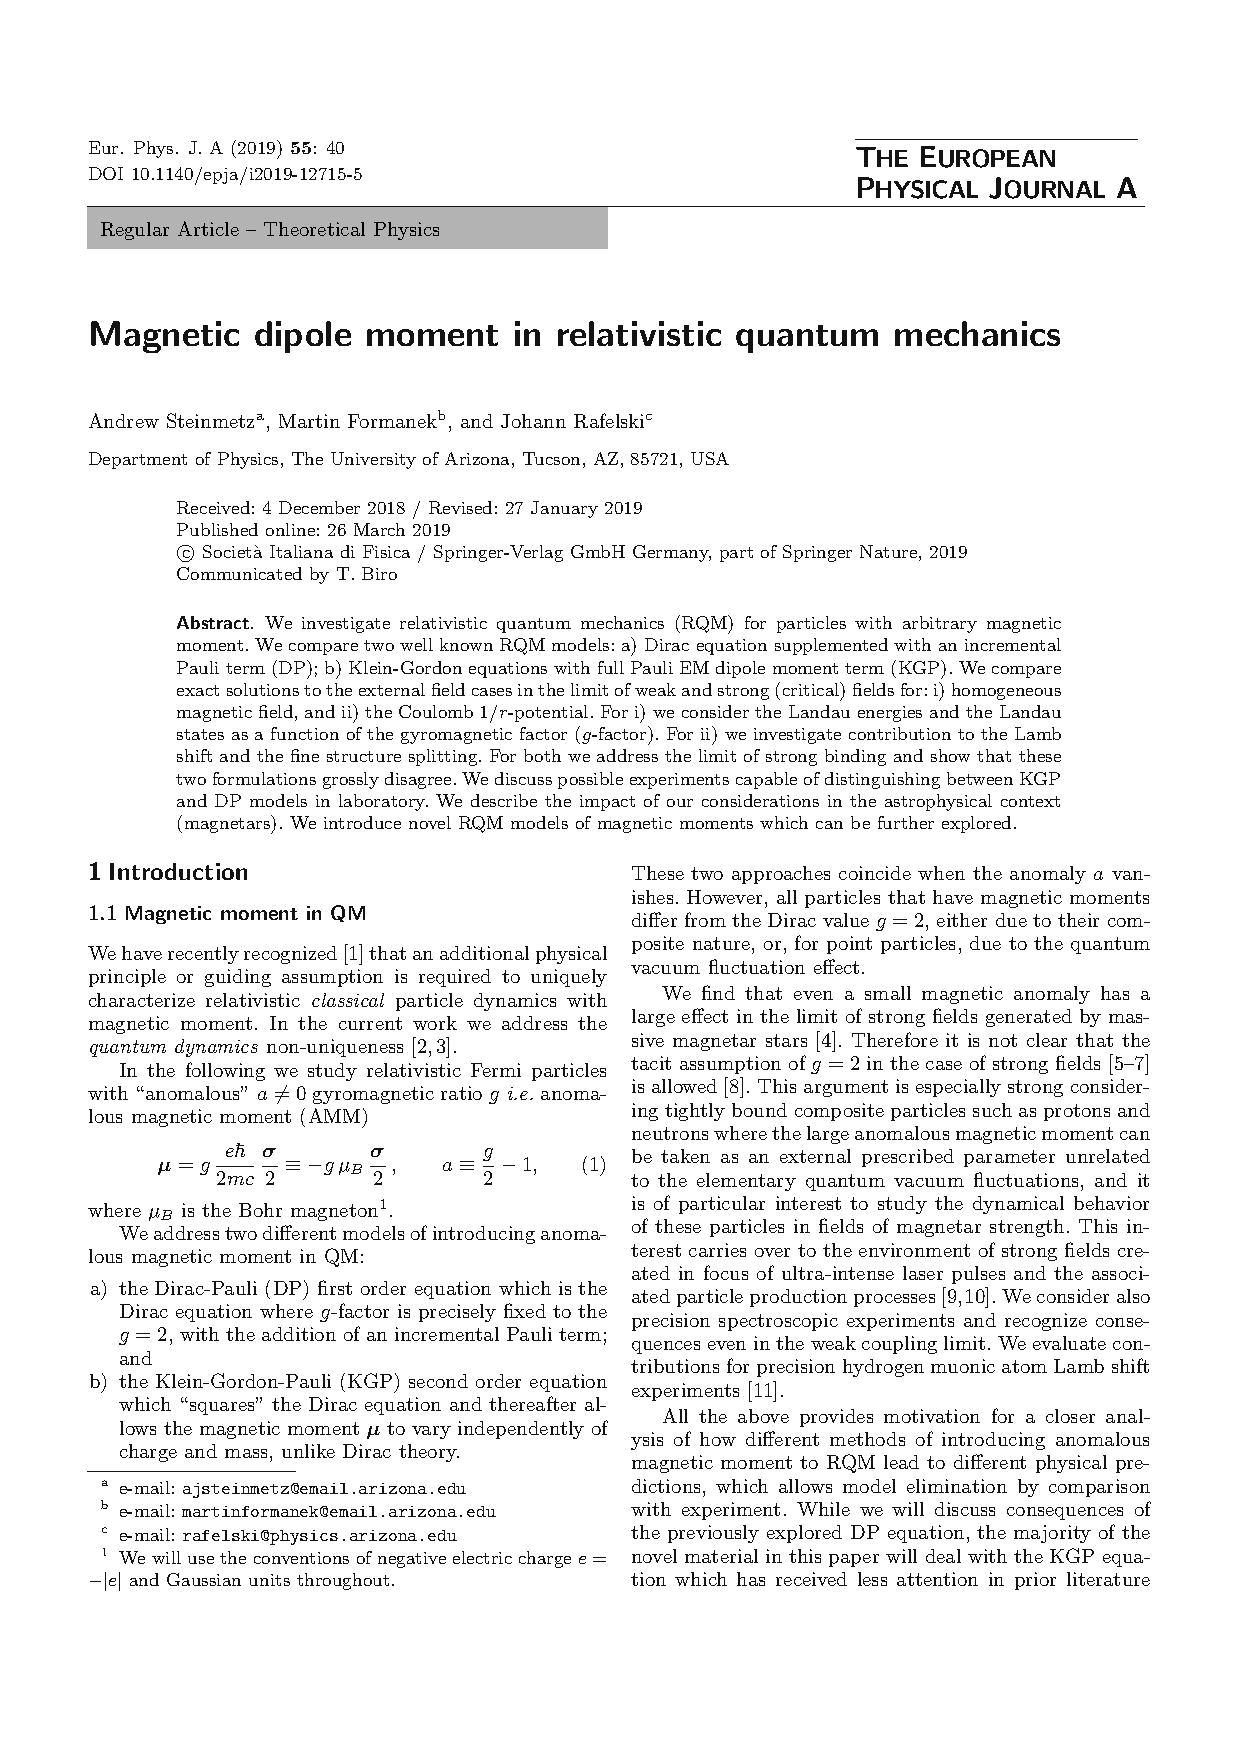
\includepdf[pages=-,pagecommand={},nup=1x2,landscape=true,width=5.5 in]{publications/steinmetz2019magnetic.pdf}

%%%%%%%%%%%%%%%%%%%%%%%%%%%%%%%%%%%%%%%
\chapter{Strong fields and neutral particle magnetic moment dynamics}
\label{appendixB}
%%%%%%%%%%%%%%%%%%%%%%%%%%%%%%%%%%%%%%%
\begin{center}
Formanek, M., Stefan, E., Rafelski, J., Steinmetz, A., Yang, C. T. Strong fields and neutral particle magnetic moment dynamics. Plasma Physics and Controlled Fusion 60, 7 (2018): 074006. \href{https://doi.org/10.1088/1361-6587/aac06a}{10.1088/1361-6587/aac06a}
\end{center}

\noindent Copyright (2018) by IOP Publishing. All rights reserved. Reproduced with permission under \href{https://marketplace.copyright.com/rs-ui-web/mp/license/56222509-d3e0-45fd-8ba6-f519e90d4d18/3a89c359-de4e-466f-93c3-ef1135413aab}{License Agreement 1384591-1} License date: August 9th, 2023. This is the Accepted Manuscript version of an article accepted for publication in Plasma Physics and Controlled Fusion. IOP Publishing Ltd is not responsible for any errors or omissions in this version of the manuscript or any version derived from it. The Version of Record is available online at \href{https://doi.org/10.1088/1361-6587/aac06a}{10.1088/1361-6587/aac06a}.

%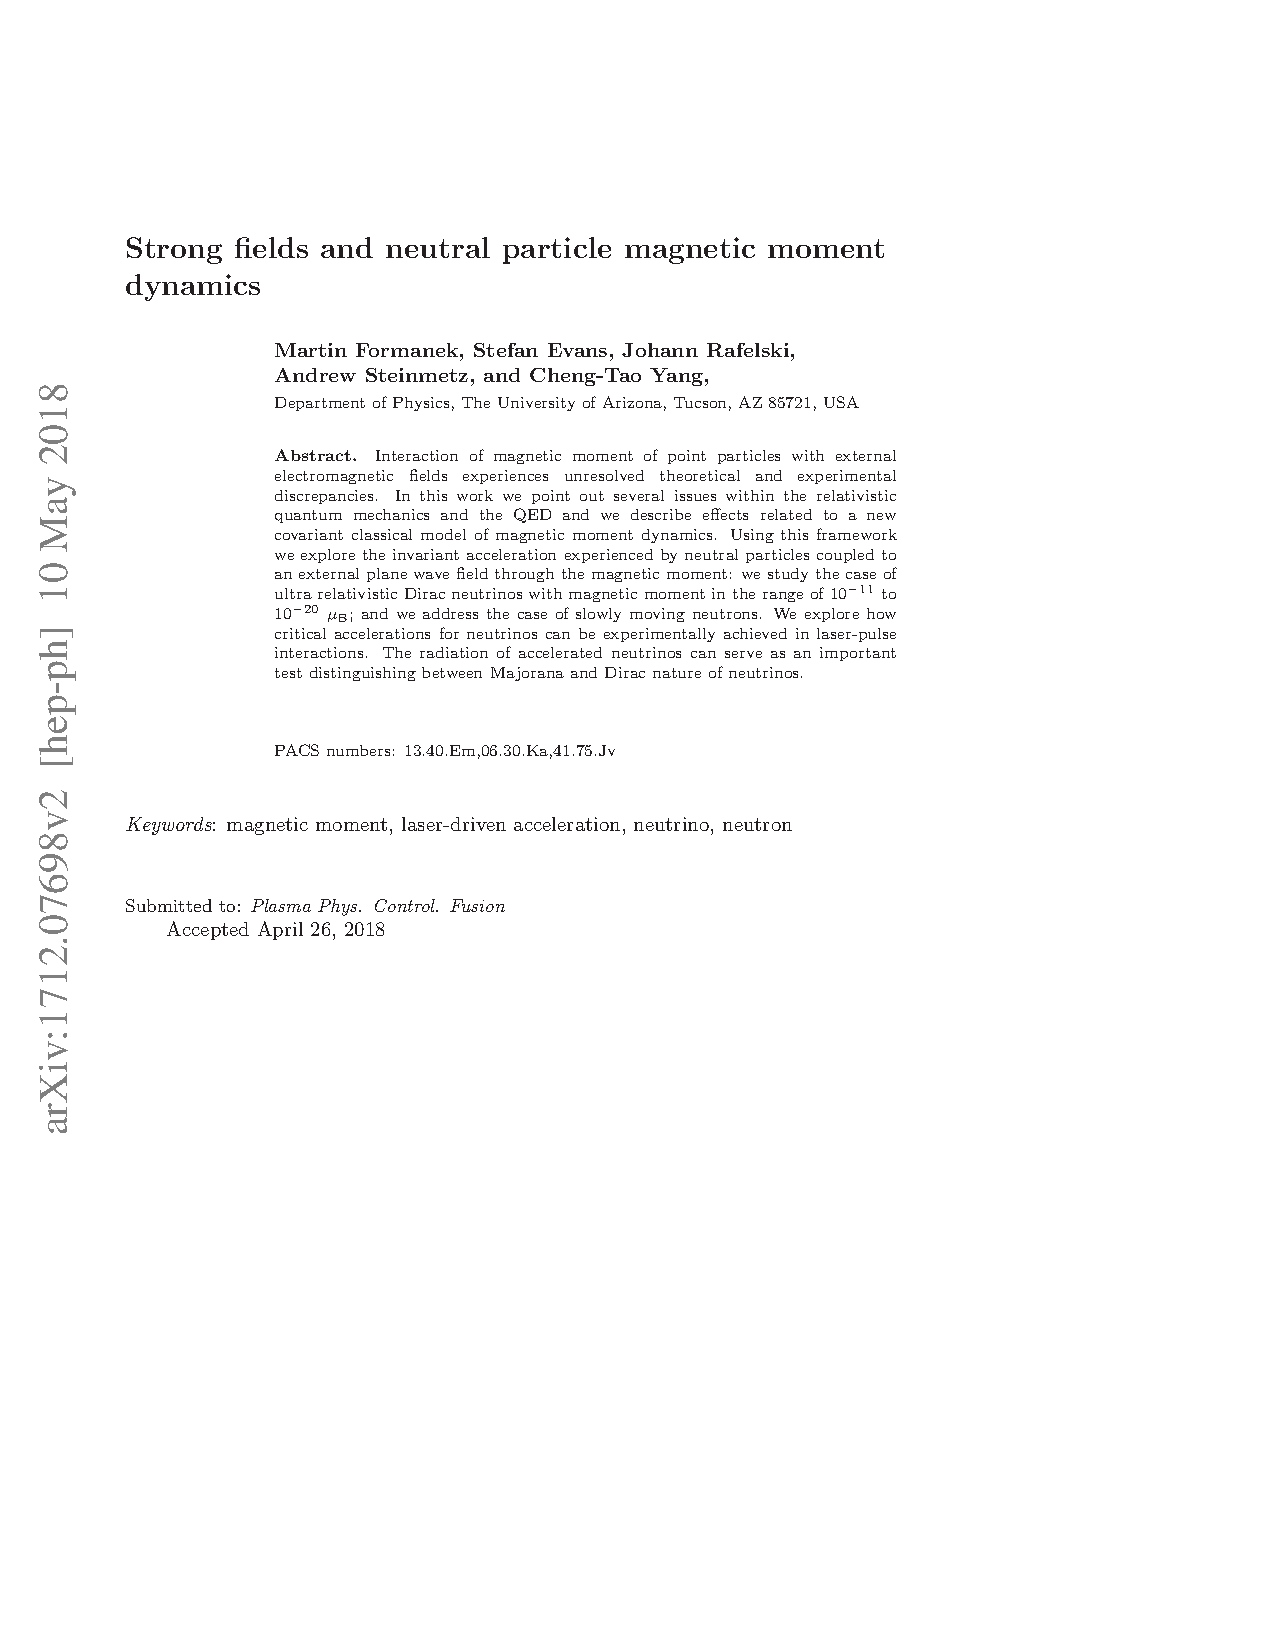
\includepdf[pages=-,pagecommand={},nup=1x2,landscape=true,width=5.5 in]{publications/formanek2018strong.pdf}

%%%%%%%%%%%%%%%%%%%%%%%%%%%%%%%%%%%%%%%
\chapter{Relativistic dynamics of point magnetic moment}
\label{appendixC}
%%%%%%%%%%%%%%%%%%%%%%%%%%%%%%%%%%%%%%%
\begin{center}
Rafelski, J., Formanek, M., Steinmetz, A. Relativistic dynamics of point magnetic moment. Eur. Phys. J. C $\bb{78}$, 6 (2018). \href{https://doi.org/10.1140/epjc/s10052-017-5493-2}{10.1140/epjc/s10052-017-5493-2}
\end{center}

\noindent Copyright (2018) by Springer Nature. Reprinted with kind permission of The European Physical Journal (EPJ). This article is an open access article distributed under the terms and conditions of the Creative Commons Attribution \href{https://creativecommons.org/licenses/by/4.0/}{(CC BY 4.0)} license.

%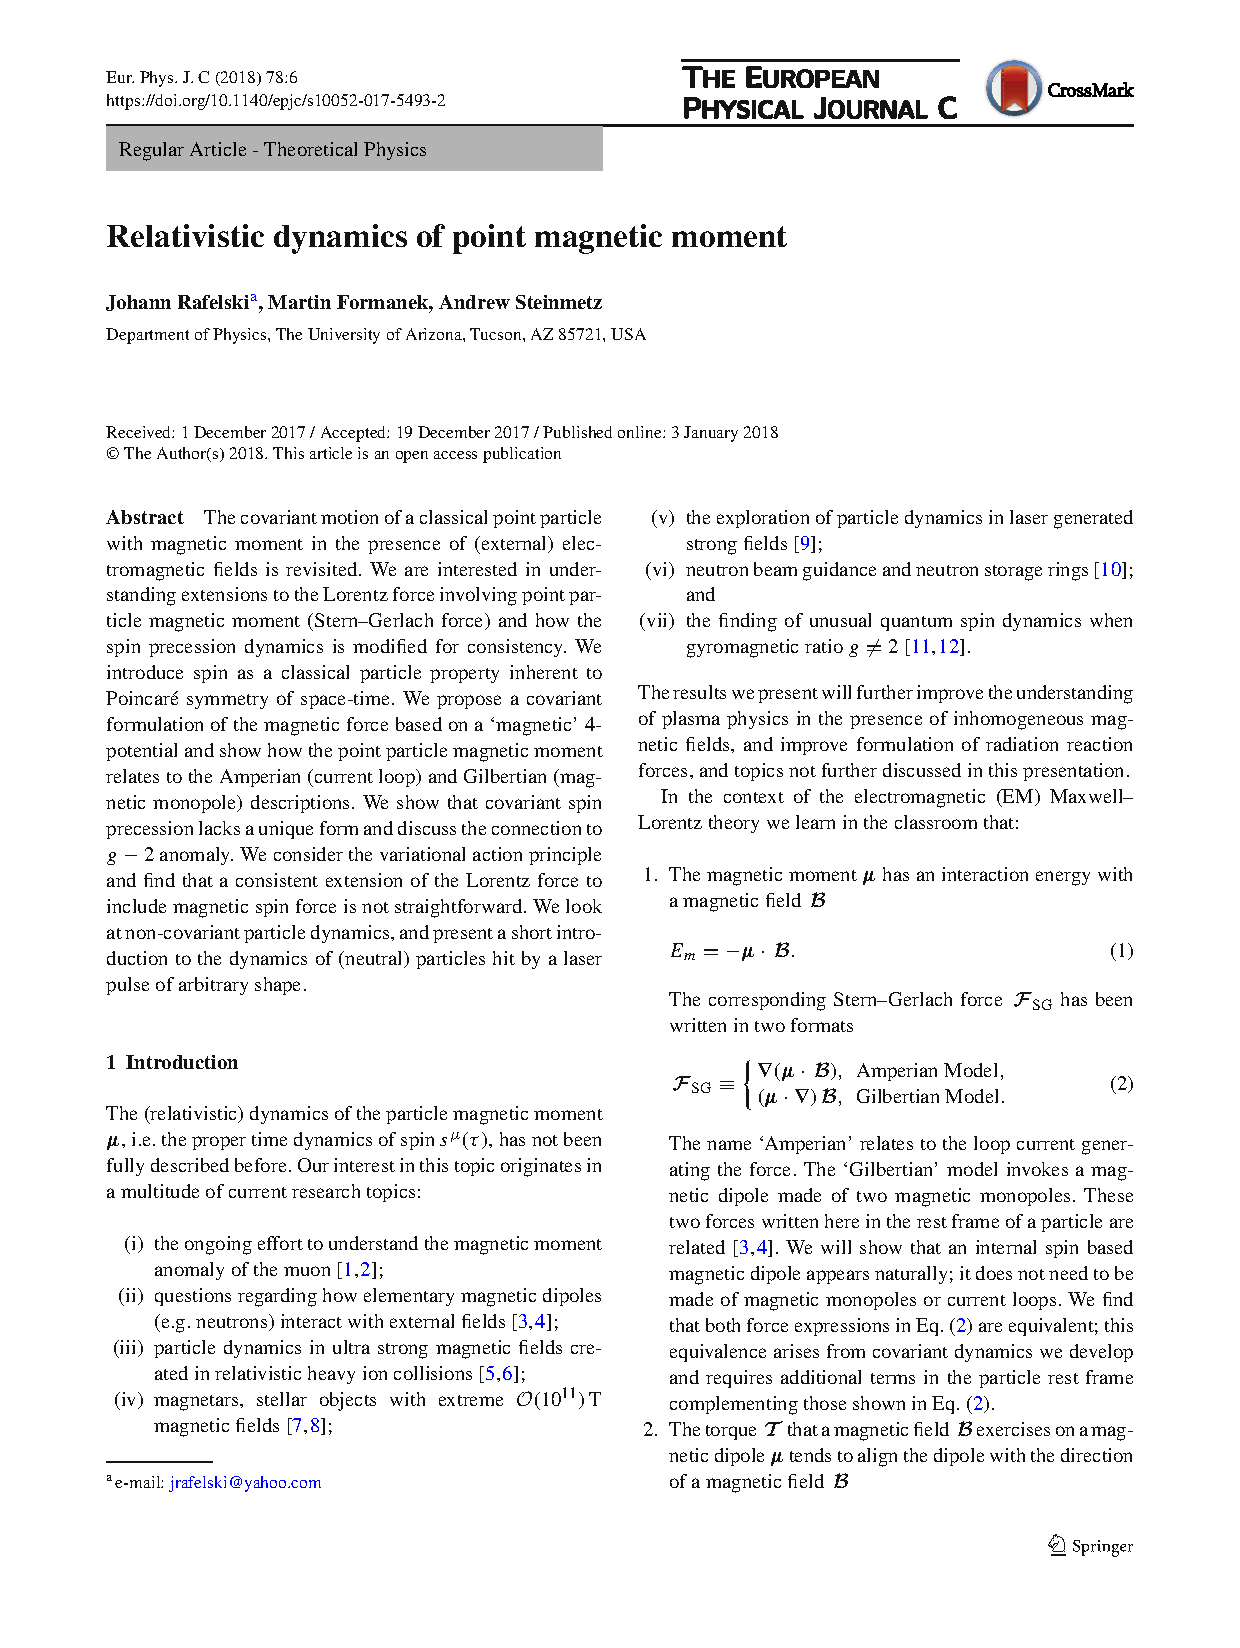
\includepdf[pages=-,pagecommand={},nup=1x2,landscape=true,width=5.5 in]{publications/rafelski2018relativistic.pdf}

%%%%%%%%%%%%%%%%%%%%%%%%%%%%%%%%%%%%%%%
\chapter{Dynamic fermion flavor mixing through transition dipole moments}
\label{appendixD}
%%%%%%%%%%%%%%%%%%%%%%%%%%%%%%%%%%%%%%%
\begin{center}
Rafelski, J., Steinmetz, A., Yang, C.T. Dynamic fermion flavor mixing through transition dipole moments. \emph{arXiv preprint}. 2023.
\end{center}

\noindent Copyright (2023) by the authors. Contribution to the book edited by Gerhard Buchalla, Dieter L\"ust
and Zhi-Zhong Xing dedicated to memory of Harald Fritzsch. Submitted an a separate article to International Journal of Modern Physics A.

%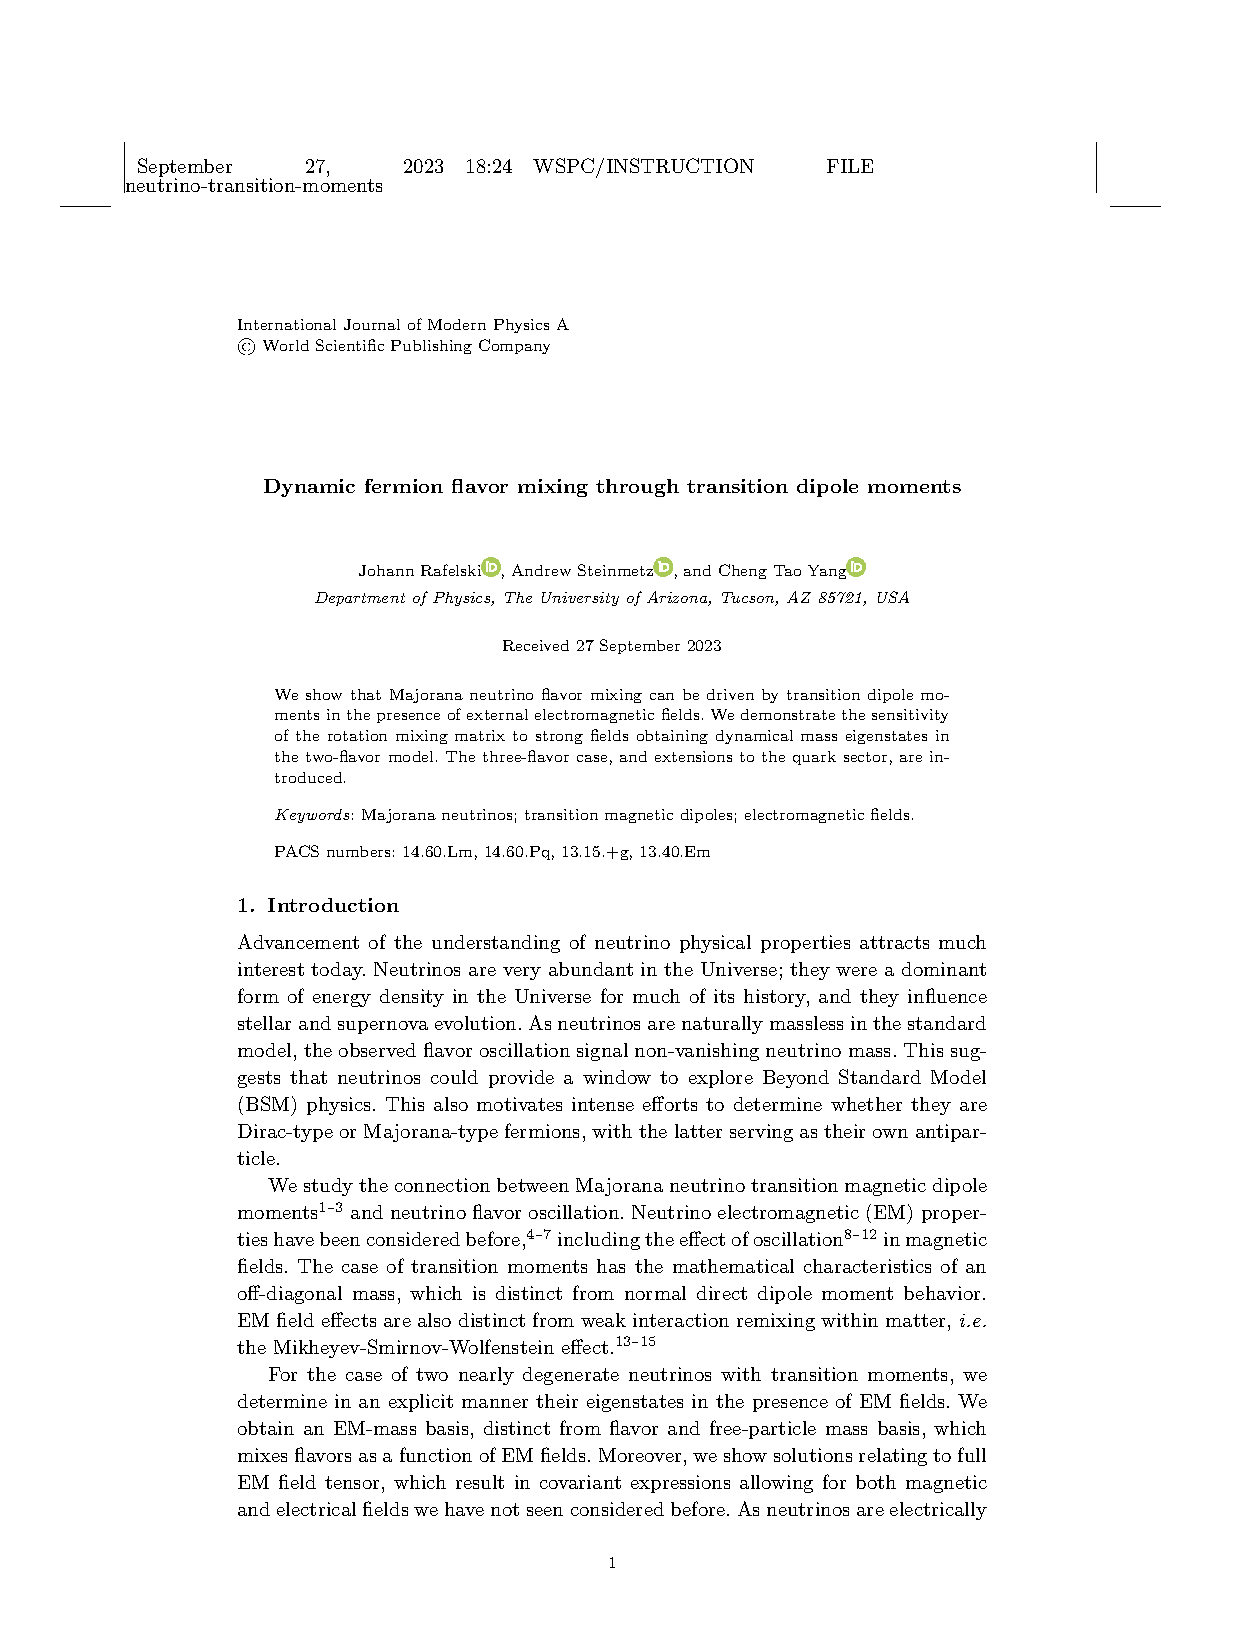
\includepdf[pages=-,pagecommand={},nup=1x2,landscape=true,width=5.5 in]{publications/rafelski2023dynamic.pdf}

%%%%%%%%%%%%%%%%%%%%%%%%%%%%%%%%%%%%%%%
\chapter{A Short Survey of Matter-Antimatter Evolution in the Primordial Universe}
\label{appendixE}
%%%%%%%%%%%%%%%%%%%%%%%%%%%%%%%%%%%%%%%
\begin{center}
Rafelski, J., Birrell, J., Steinmetz, A., Yang, C.T. A Short Survey of Matter-Antimatter Evolution in the Primordial Universe. Universe 2023, 9, 309. \href{https://doi.org/10.3390/universe9070309}{10.3390/universe9070309}
\end{center}

\noindent Copyright (2023) by the authors. Licensee MDPI, Basel, Switzerland. This article is an open access article distributed under the terms and conditions of the Creative Commons Attribution \href{https://creativecommons.org/licenses/by/4.0/}{(CC BY 4.0)} license.

%\includepdf[pages=-,pagecommand={},nup=1x2,landscape=true,width=5.5 in]{publications/rafelski2023shortsurvey.pdf}

%%%%%%%%%%%%%%%%%%%%%%%%%%%%%%%%%%%%%%%
\chapter{Matter-antimatter origin of cosmic magnetism}
\label{appendixF}
%%%%%%%%%%%%%%%%%%%%%%%%%%%%%%%%%%%%%%%
\begin{center}
Steinmetz, A., Yang, C.T. \& Rafelski, J. Matter-antimatter origin of cosmic magnetism. \emph{arXiv preprint}. 2023. \href{https://arxiv.org/abs/2308.14818}{arXiv:2308.14818 [hep-ph]}
\end{center}

\noindent Copyright (2023) by the authors. Submitted to Physical Review D.

%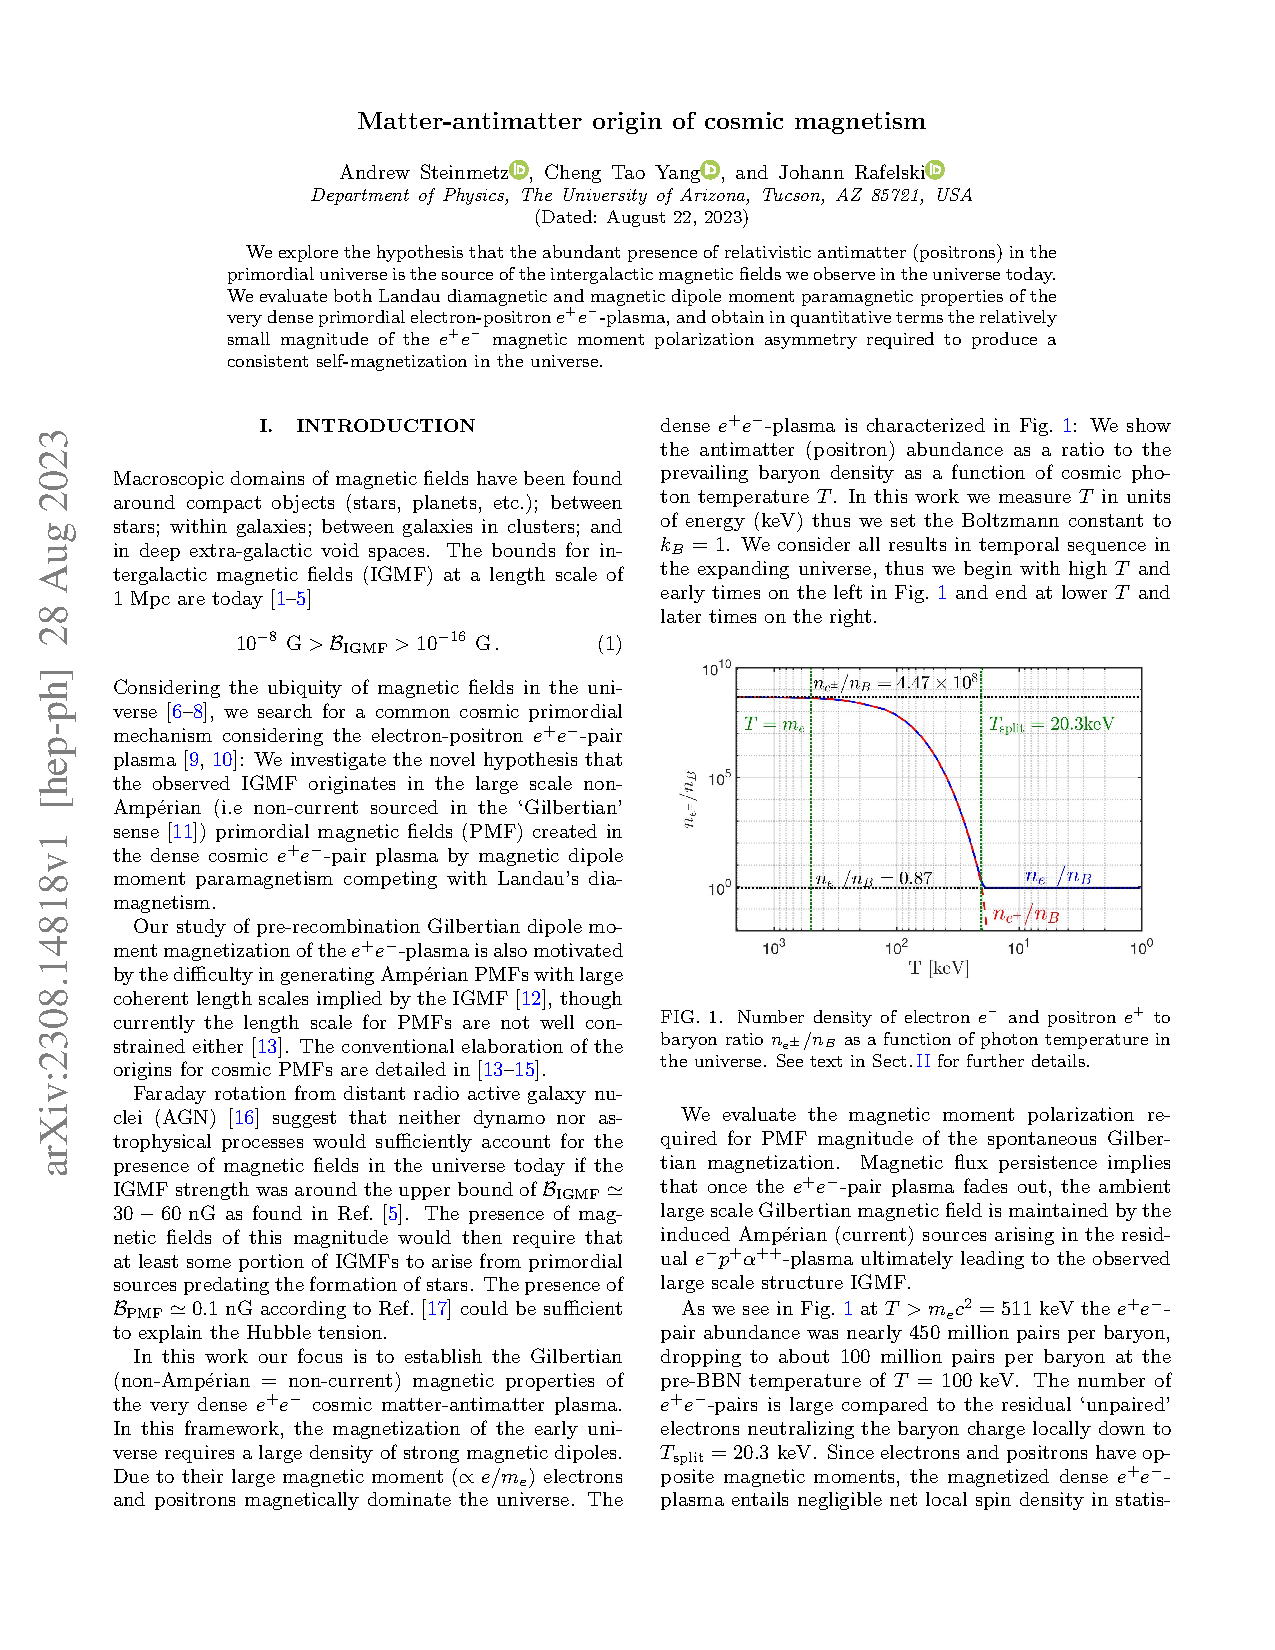
\includepdf[pages=-,pagecommand={},nup=1x2,landscape=true,width=5.5 in]{publications/steinmetz2023matter.pdf}
